\setcounter{chapter}{4}
\chapter{Elettrodinamica}

\section{Leggi d'induzione}

Lo studio delle trasformazioni del campo elettrostatico e del campo magnetico stazionari in sistema in moto relativo ha evidenziato che $\bold{E}$ e $\bold{B}$ sono in un qualche modo legati tra loro.

In fenomeni variabili (dipendenti dal tempo) $\bold{E}$ e $\bold{B}$ sono mutuamente accoppiati. Alcune relazioni che descrivono i campi stazionari sono incomplete e vanno estese.
Se consideriamo una carica puntiforme in moto nel sistema di riferimento del laboratorio, allora le seguenti leggi dedotte per le cariche statiche non sono pi\`u valide:
\begin{align*}
	& \bold{E} \quad \text{non \`e conservativo} \iff \nabla \times \bold{E} \neq 0 \\[0.3cm]
	& \bold{B} \quad \text{non soddisfa la legge di Amp\`ere } \iff \nabla \times \bold{B} \neq \mu_0 \bold{J}
\end{align*}
Iniziamo l'analisi dei fenomeni non stazionari dalle osservazione sperimentali di Faraday che sistemano la prima relazione $\nabla \times \bold{E} \neq 0$.  Data una carica statica all'interno di un conduttore 
questa induce una carica indotta nei conduttori, ma che cosa succede se una corrente di carica atteaversa un conduttore ? speriementalmente si osserva una corrente indotta al suo interno per flussi vairabili nel tempo. Ma a questo punto diventa 
leggittimo domandarsi come mai le cariche all'interno del conduttore si mettano in moto, ovvero quali siano le forze (apparenti) responsabili?

Inoltre Faraday compie altri esperimenti che restituiscono il medesimo risultato:
\begin{enumerate}
	\item conduttore deformato o in movimento immerso in un campo elettromagnetico $\bold{B}$ stazionario;
	\item le sorgenti del campo magnetico $\bold{B}$ sono in moto rispetto al coduttore;
	\item conduttore in presenza di campo magnetico variabile della sorgente
\end{enumerate}

\subsection{Esempio}

Consideriamo un conduttore dato da una spira quadrate nel piano (x,y). Definiamo un sistema di riferimento solidale con la spira $S_Q$ e un sistema  O in cui si trova l'osservatore. La spira si muove con una velocit\`a $\bold{v_c}$ rispetto ad O. 
\begin{center}
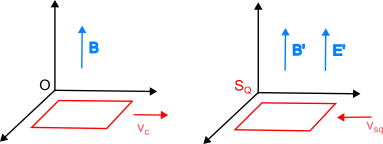
\includegraphics[width = 0.6 \textwidth]{images/relati.png}
\end{center}

Nella prima immagine partendo da sinistra abbiamo che 
\begin{equation}
	\bold{F_B} = q\bold{v_c} \times B \neq 0  
\end{equation}
mentre il campo elettrico \`e $E = 0 $. Da questo risultato possiamo dedurre che la corrente indotta che si osserva all'interno della spira deve essere conseguenza di una forza di natura magnetica. 

Se consideriamo la seconda immagine in cui $S_Q$ \`e  il sistema fissato, osserveremo il sistema O muoversi con velocit\`a $\bold{v_c}$ in senso opposto. Rispetto al sistema  $S_Q$ le cariche sono stazionare 
di conseguenza $F_{B'} = 0$ e quindi la corrente che si osserva all' interno della spira non pu\`o essere conseguenza di un effetto magnetico. Inoltre \`e presente un campo eletrico $E'$.

Nel seguente paragrafo delineiamo i principi che legano il campo magnetico variabile alle forze che permettono di osservare della corrente all'interno di un conduttore.
\section{Legge di Faraday}

Una delle equazioni di Maxwell mette in relazione campi magnetici ed elettrici 
\begin{equation}
	\nabla \times \bold{E} + \frac{\partial \bold{B}}{\partial t} = 0
\end{equation}
Tale equazione ci dice che che se il campo magnetico \`e variabile nel tempo, allora crea un campo elettrico. La creazione di un campo elettrico fa s\`i che le cariche vengano accelerate, ovvero creino una corrente all'interno di un filo. Il processo di creazione di una corrente mediante un campo magnetico variabile prende il nome di \textit{induzione}.

\begin{wrapfigure}{r}{0.4\textwidth} % 'r' for right, 'l' for left
    \centering
    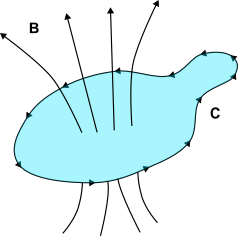
\includegraphics[width=0.32\textwidth]{images/faraday_law}
\end{wrapfigure}
Consideriamo un filo come un conduttore, avvolto attorno ad una curva stazionaria C. Un filo chiuso prende il nome di circuito. Se integriamo l'equazione (5.1) rispetto alla superficie S racchiusa dal circuito chiuso C, abbiamo che
\begin{equation*}
	\int_{S}(\nabla \times \bold{E}) \cdot d \bold{S} = - \int_{S} \frac{\partial \bold{B}}{\partial t} \cdot d\bold{S}
\end{equation*}
utilizzando il teorema di Stokes possiamo riscrivere l'equazione come
\begin{equation*}
	\oint_{C} \bold{E} \cdot d\bold{r} = - \int_{S} \frac{\partial \bold{B}}{\partial t} \cdot d \bold{S} = - \frac{d}{dt} \int_{S} \bold{B} \cdot d \bold{S}
\end{equation*}
Per ottenere l'ultima relazione abbiamo assunto che n\`e C e n\`e S possano cambiare nel tempo. L'integrale di linea attorno a C del campo elettrico prende il nome di \textit{forza elettromotrice}, $\mathcal{E}$, che di solito viene abbreviata con $fem$.
\begin{equation*}
	\mathcal{E} = \oint_{C} \bold{E} \cdot d \bold{r}
\end{equation*}
La forza elettromotrice non \`e realmente una forza come possiamo vedere dalla sua espressione, in realt\`a \`e la componente tangenziale della forza per unit\`a di carica, integrata lungo un filo. Un altro modo di vederla \`e dato dal lavoro necessario a spostare una carica unitaria lungo la curva C. Se la $fem$ \`e non nulla allora \`e presente della carica accelerata all'interno del filo che genera quindi una corrente.

L'integrale del campo magnetico passante attraverso la superficie S prende il nome di flusso magnetico $\Phi$ attraverso la superficie S,
\begin{equation*}
	\Phi = \int_{S} \bold{B} \cdot d\bold{S}
\end{equation*} 
Di conseguenza possiamo riscrivere l'equazione di Maxwell (5.1) come 
\begin{equation}
	\mathcal{E} = - \frac{d\Phi}{dt}
\end{equation}
In questa forma l'equazione prende il nome di \textit{legge di Faraday}. 
\newline

\noindent La legge di Faraday ci dice che se cambiamo il flusso del campo magnetico attraverso una superficie S delimitata da un circuito, allora osserveremo un flusso di corrente all'interno del filo. Esistono diversi modi per modificare il campo magnetico, per esempio spostando una barra magnetica in vicinanza ad un circuito, passandola attraverso la superficie S delimitata dal filo conduttore. Un altro modo \`e dato muovendo un secondo filo $C''$ attraverso da una corrente, oppure tenendolo fisso e variando l'intensit\`a di corrente al suo interno accendendolo e spegnendolo. Tutti questi metodi inducono una corrente in C.
\newline

Esiste anche un secondo effetto, dovuto al fatto che dato un campo magnetico variabile e avendo una corrente indotta all'interno del circuito C, avremo che a sua volta la carica in moto genera un suo campo magnetico. Il campo magnetico indotto \`e orientato sempre in opposizione al cambiamento. Questo fenomeno prende il nome di \textit{legge di Lenz} e giustifica il segno negativo nella legge di Faraday (5.2). 

\subsection{Esempio legge di Lenz}

\begin{wrapfigure}{r}{0.4\textwidth} % 'r' for right, 'l' for left
    \centering
    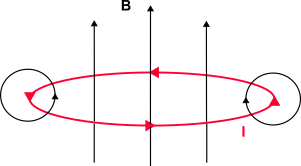
\includegraphics[width=0.38\textwidth]{images/lenz_law}
\end{wrapfigure}
Possiamo dimostrare la legge di Lenz con un semplice esempio. Consideriamo un caso in cui il cammino C \`e una circonferenza giacente in un piano, e ipotizziamo che sia immersa in campo magnetico B uniforme che al passare del tempo questo diventa pi\`u piccolo e dunque $\dot{\Phi} < 0$. Per la legge di Faraday abbiamo che $\mathcal{E} > 0 $ e la corrente scorre in senso antiorario lungo C. La corrente indotta genere una campo $\bold{B}$ che incrementa il campo all'interno della spira opponendosi alla sua decrescita.

\subsection{Esempio: Batteria (Corrente Stazionaria)}

Quando osserviamo della corrente all'interrno di un circuito ci sono solo  due forze responsabili del trasporto delle cariche: la sorgente, $\bold{F_s}$, che solitamente  \`e confinata in una porzione del circuito (come una batterria) e una forza di natura elettrostatica, che serve a trasportare l'effetto della sorgente sul  resto del circuito:
\begin{equation}
	\bold{F} = \bold{F_s}  + \bold{E}
\end{equation}
Nel caso di una batteria $\bold{F_s}$ \`e data dal potenziale chimico al suo interno. Il lavoro compiuto complessivamente sul circuito \`e dato come sempre dall'integrale di linea della forza agente su di esso quindi 
\begin{equation*}
	\mathcal{E} \equiv \int_{C} \bold{F} \cdot \bold{ds} = \int_C  \bold{F_s}  \cdot \bold{ds}
\end{equation*}

e quindi come definito il precedente all'interno del circuito  abbiamo una forza elettromotrice responsabile de flusso delle cariche al suo iterno.  

Se consideriamo un modello semplificato della batteria, in cui ne trascuriamo la resistenza,  abbiamo che la forza sulle cariche \`e  $E = -\bold{F_s} $, dunque la \textit{fem} possiamo vederla legata alla tensione ai campi della batteria.
\begin{equation*}
	\mathcal{E} = \int_{C} \bold{F_s} \cdot \bold{ds} = - \int_{a}^b \bold{E} \cdot \bold{dl} = V
\end{equation*}

Lo scopo di una batteria \`e  quelllo di manterna un differza di potenziale all'internro di un circuito pari alla forza elettromotrice. Notare che all'interno di una batteria $\bold{F_s}$ la corrente ha flusso in direzione opposta al campo elettrico $\bold{E}$.
 \newpage

\subsection{Generatori Elettrici}

Ipotizziamo di avere un sistema in cui abbiamo una sorgente (generatore) che genera un campo magnetico $\bold{B}$ stazionario, ma non uniforme nello spazio. Nel sistema \`e presente una spira rettangolare in moto con velocit\`a $\bold{v}$ costante.

\begin{center}
	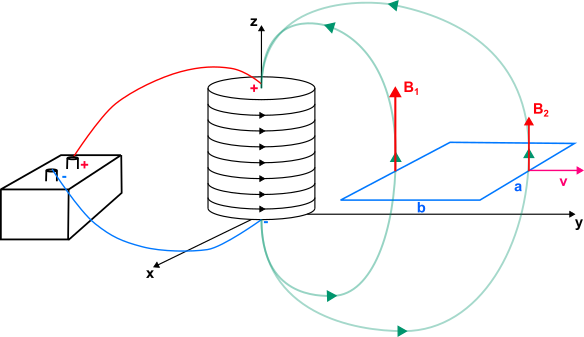
\includegraphics[width = 0.6 \textwidth]{images/generator.png}
\end{center}

Siccome il campo magnetico $\bold{B} = \bold{B}(\bold{r})$ dipende dalla poszione la forza a cui sono soggette le cariche nella spira dipende dalla distanza dalla sorgente. Calcolando la forza di Lorenetz  per unit\`a di carica  $\bold{F_B} = \bold{v} \times \bold{B}$, ad un istante di tempo t:
\begin{equation*}
	\oint \bold{F_B} \cdot \bold{ds} = v(B_1 - B_2)a \neq 0 
\end{equation*}
dove $a$ \`e la lunghezza di un tratto della spira.  Lungo $b$ la forza $\bold{F_B}$ \`e ortogonale al tratto di spira (vedere figura) di conseguenza non contribusce all'intergrale, e quindi si un constributo solo lungo $a$ dove $\bold{F_B}$ \`e parallelo alla direzione.

La forza complessiva che agisce su una carica  del circuito \`e data da 
\begin{equation*}
	\bold{F} = q \bold{v} \times \bold{B} + q\bold{E}
\end{equation*}

di conseguenza il lavoro compiuto dal generatore \`e dato da 
\begin{equation*}
	\mathcal{E} = \oint \bold{f} \cdot \bold{ds} = \oint (\bold{v} \times \bold{B} + \bold{E}) \cdot \bold{ds} = \oint (\bold{v} \times \bold{B}) \cdot \bold{ds}
\end{equation*}
dove si \`e trascurato il contributo del campo elettrico $\bold{E}$ essendo conservativo. Il lavoro compiuto dal generatore \`e  proprio la forza elettromotrice che permette lo spostamento delle carriche e coincide con la forza di Lorentz per unit\`a di carica.

\subsection{Moto di un filo in un campo magnetico stazionario}

Come abbiamo visto un modo per indurre una corrente all'interno un conduttore \`e  quello di mantere la sorgente fissata e il conduttore in moto. Se prendiamo come conduttore una barra di lunghezza $a$ (o segmento di circuito), le cariche libere si muovono sotto l'azione di $\bold{F_B} = q \bold{v} \times \bold{B}$.
sulle cariche si raggiunge uno stato di equilibrio statico quondo il campo $\bold{E}$ interno al conduttore, generato dalla distribuzione di carica, ottenuta doopo il riarrangiamento indotto da $\bold{F_B}$, bilancia la forza di Lorentz.
\begin{equation*}
	\bold{F_B} + \bold{F_E} = 0 \iff \bold{E} = - (\bold{v} \times \bold{B})
\end{equation*}  
Ai capi della barra compare una differenza di potenziale

\begin{equation*}
	\Delta V  = - \int_{0}^{a} \bold{E} \cdot \bold{ds} = \int_0^{a}(\bold{v} \times \bold{B}) \cdot \bold{ds}
\end{equation*}

Se il circuito \`e chiuso, se $\bold{B}$ non \`e uniforme, abbiamo che $\Delta V_1 \neq \Delta V_2$ nei due segmenti distanti tra loro, di conseguenza compare una $fem$, dovuta alla forza di Lorentz.

\subsection{Lavoro della forza esterna }

Prendiamo un sistema in cui \`e presente un campo magnetico $\bold{B}(\bold{r})$ non uniforme e al suo interno \`e  immersa una spira rettangolare di lato minore $a$ (il lato maggiore non ci interessa per la dinamica del problema). Ipotizziamo che la spira sia tirata da una forza esterna $\bold{F_ext}$ concorde con gli assi del 
sistema di riferimento. All'interno della spira \`e presenta una corrente di cariche che si spostano con velocit\`a $\bold{v}_D$ che \`e la velocit\`a di deriva e una componente di velocit\`a $\bold{v}$ data dalla forza esterna agente. La velocit\`a di una singola carica \`e quindi data da
\begin{equation*}
	\bold{v}_q =  v_D \bold{\hat{\mu}_x}  + v \bold{\hat{\mu}_y}
\end{equation*}

La forza sulle cariche presenti nei due segmenti verticali alla direzione di spostamento che contribuiscono al lavoro \`e data da 
\begin{equation*}
	\bold{F_1} = q \bold{v} \times \bold{B_1} = \underbrace{-q \bold{v_D}B_1 \bold{\hat{\mu}_y}}_{\text{opposta a } \bold{F_{ext}} } + qvB_1 \hat{\mu}_x
\end{equation*}

il secondo addendo determina il moto delle cariche nel filo.